\documentclass[11pt, xcolor=table]{beamer}
\usetheme{Singapore}

\usepackage[utf8]{inputenc}
\usepackage[T1]{fontenc}
\usepackage{soul}
\usepackage{graphicx}
\usepackage[normalem]{ulem}
\useunder{\uline}{\ul}{}

\graphicspath{{../../Figures/}}

\def\et{{\it et al.}}


\author{Cody Glickman  \\ CPBS Update Talk}

\title{Metagenomic Exploration the Sequel: \\ Development of tools for viral and bacterial sequence analysis}

%\subtitle{}
%\logo{}

\date{ 
\includegraphics[height=2cm, width=2cm]{lablogo.png} \\ Nov 12th, 2018}
%\subject{}
\setbeamercovered{transparent}
\setbeamertemplate{navigation symbols}{}
\setbeamertemplate{theorems}[numbered]

\begin{document}
	\maketitle

  %------------------------------------------------------------------ Outline
	\begin{frame}{Research Update Outline}
	\begin{block}{Virulence Factors in Bacteriophages}
	\tiny{Glickman C., Hendrix J., Strong M. Computational identification and analysis of bacterial virulence factors embedded into bacteriophage genomes. Poster session accepted at: Rocky 18: 2018 Dec 8-10; Snowmass, CO}
	\end{block}
	
	\begin{block}{Building Up Domains: Lysogenic Host Discovery}
  Incorporated into NCBI's Virus Discovery Project
	\end{block}

	\begin{block}{Hybrid Viral Metagenome Prediction}
	\tiny{Glickman C., Strong M. Hybrid Viral Identification in Metagenomics. In preperation: Early 2019}
	\end{block}
	\end{frame}
	%------------------------------------------------------------------
	\begin{frame}{Progress of Other Projects}
	\begin{block}{Asthma Environmental Microbiome}
	\tiny{Koon P., Glickman C., Epperson L.E., Strong M., Clemente J.C., Vicencio A., Diette G., Bose S. Household determinants of the indoor environmental microbiome in an urban asthmatic population. Poster submitted: ATS 2019: 2019 May 17-22; Dallas, TX}
 
	\end{block}
	
		
	\begin{block}{Clinical NTM Gene Databases}
	\tiny{Glickman C., Epperson L.E., Hasan N., Strong M. Clinical NTM Gene Database. In preperation: Late 2018}
	\end{block}
	
	\begin{block}{Duobiome: 18S/16S Parallel Analysis}
	\tiny{Glickman C., Russell P., Epperson L.E., Strong M. DuoBiome: A workflow for mixed metagenomes. In preperation: Early 2019}
	\end{block}
	
	
	\begin{block}{Genomic Retrieval and Blast Database Creation}
	\tiny{Glickman C., Strong M. Batch retrieval and BLAST database creation tool. Poster session accepted at: Modelling microbial communities and functions. ISME 17: 2018 Aug 12-17; Leipzig, Germany}
	\end{block}
	
	\begin{block}{Hawaiian Soil Chemistry and Culture}
	\tiny{Glickman C., Virdi R., Epperson L.E., Strong M., Nelson S., Honda J. Relationship Between Soil Mineral Characteristics and Non-Tuberculosis Mycobacterium Growth. In preperation: Early 2019}
	\end{block}
	

	\end{frame}
	%-----------------------------------------------------------
\section{}


	\begin{frame}{Nontuberculous Mycobacterial (NTM) Infections}
	  
		\begin{block}{Number of Cases}
		The number of NTM cases is estimated over 100K
		\end{block}
		
		\begin{block}{Increasing Case}
		The rate of cases is estimated to grow at 8\% every year
		\end{block}
		
		
		\begin{block}{Populations at risk of developing NTM}
		\begin{itemize}
		\item Immunocompromised individuals 
		\item Patients with lung damage or malfunction 
		\item Residents of warm costal areas especially Hawaii
		%\item The Elderly 
		\end{itemize}
		\end{block} 
		
		\begin{block}
		
		\end{block}
	\vspace{-1cm}
	\tiny{Strollo SE, et al. Ann Am Thorac Soc. (2015) \\
	Adjemian J, et al. Am J Respir Crit Care Med. (2012)}
	
	\end{frame}
	%----------------------------------------------------------

	\begin{frame}{Viral Focus}
	\begin{columns}
	\column{0.5\textwidth}
	\begin{block}{Bacteriophages (Phages)}
	Phages are DNA viruses that infect prokaryotes
	\end{block}
	
	\begin{block}{Phage Diversity}
	How phage abundance and diversity effects susceptibility to NTM lung infection
	\end{block}
	
	\begin{block}{Phages as Vectors}
	How phages carry bacterial genes within clinical NTM infections
	\end{block}
	
	
	\column{0.5\textwidth}
	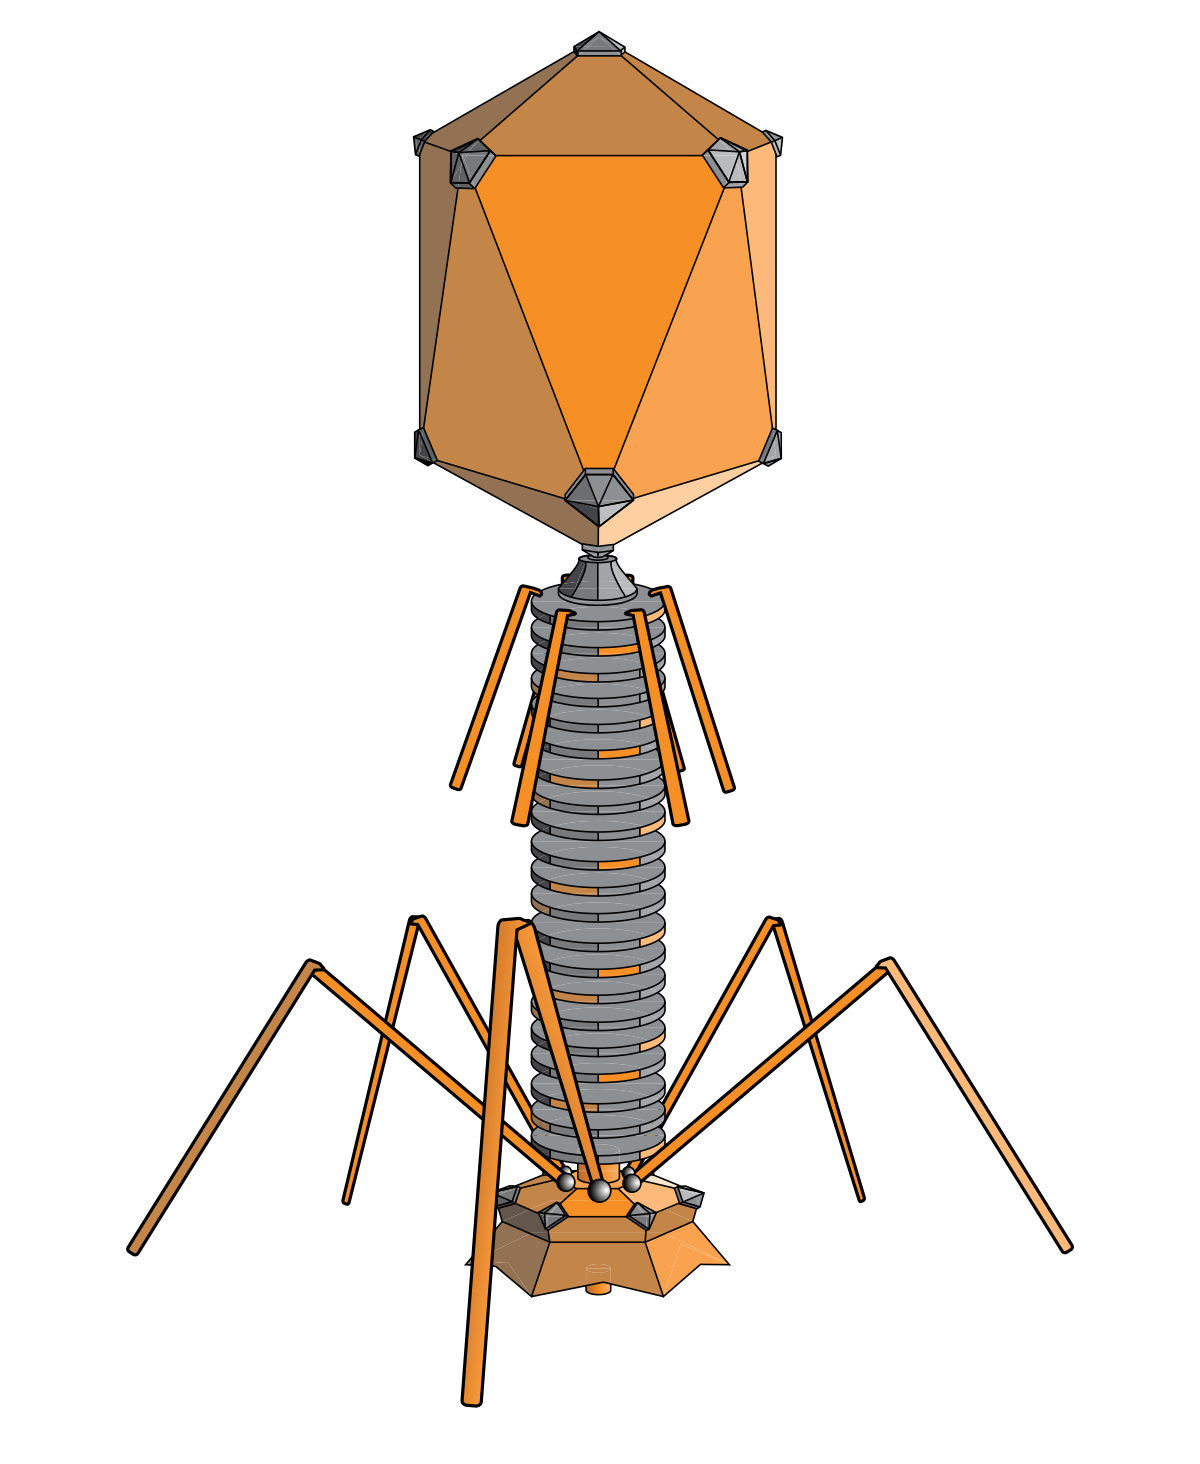
\includegraphics[height=5.5cm, width=5cm]{phage.png} \\
	\end{columns}
	
	
	\end{frame}
	%-----------------------------------------------------------

	\begin{frame}{Objective}
	\center
	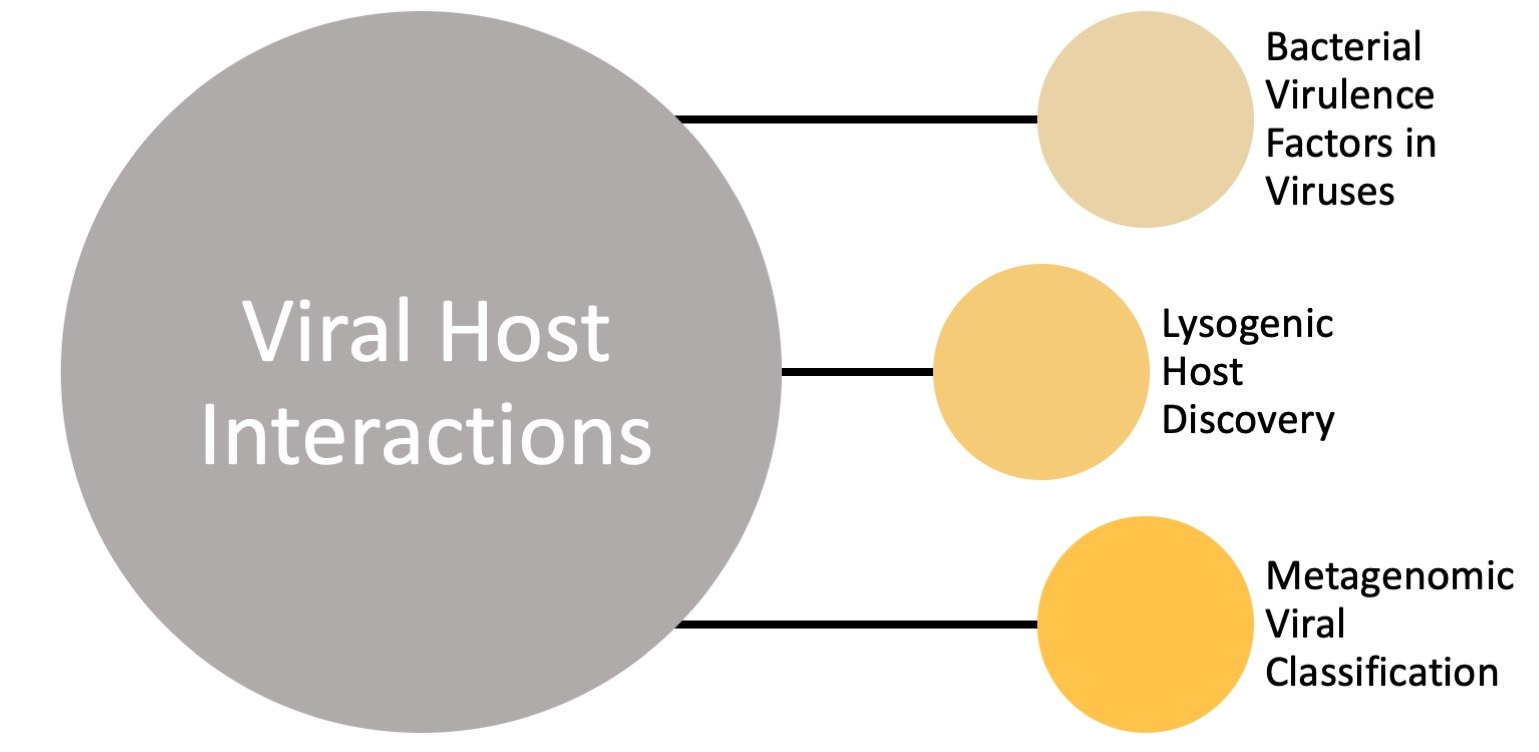
\includegraphics[height=6cm, width=10cm]{CPBS_11_18/Overview.jpg}
	
	\end{frame}

%-----------------------------------------------------------
	

\section{}
%------------------------------------------------------------------ Outline
	\begin{frame}{Research Update Outline}
	\begin{block}{Virulence Factors in Bacteriophages}
	\tiny{Glickman C., Hendrix J., Strong M. Computational identification and analysis of bacterial virulence factors embedded into bacteriophage genomes. Poster session accepted at: Rocky 18: 2018 Dec 8-10; Snowmass, CO}
	\end{block}
	
	\begin{block}{\textcolor{black!50}{Building Up Domains: Lysogenic Host Discovery}}
  \textcolor{black!50}{Incorporated into NCBI's Virus Discovery Project}
	\end{block}

	\begin{block}{\textcolor{black!50}{Hybrid Viral Metagenome Prediction}}
	\textcolor{black!50}{\tiny{Glickman C., Strong M. Hybrid Viral Identification in Metagenomics. In preperation: Early 2019}}
	\end{block}
	\end{frame}
%------------------------------------------------------------------
\section{Virulence Factors in Phages}
\subsection{}
	
	\begin{frame}{Virulence}
		\begin{block}{Virulence Defined}
		The capacity of a microorganism to proliferate despite host defenses
		\end{block}
		
		\begin{block}{Influences on Virulence}
		\begin{itemize}
		\item Number of microorganisms
		\item \alert{Composition of the mobile genetic reservoir}
		\item Location of niche
		\item Host immune capabilities
		\end{itemize}
		\end{block}
	
	\end{frame}
	%--------------------------------------------------------------------------------------


	
	%--------------------------------------------------------------------------------------
	
	\begin{frame}{Phages as a Genetic Reservoir \\ of Virulence Factors Genes}
	\begin{columns}
	\column{0.5\textwidth}
	\vspace{-1cm}
	\begin{block}{Phages and Pathology}
	Virulence factors that cause cholera, dysentery, botulism, and food poisoning are carried on phage elements
	\end{block}
	
	\column{0.5\textwidth}
	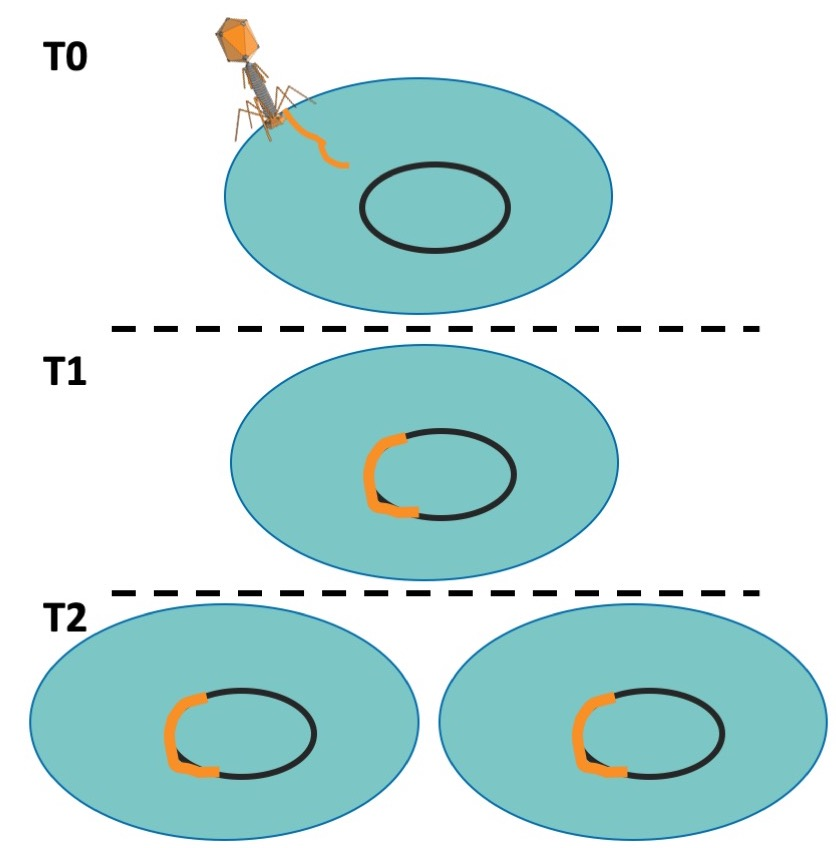
\includegraphics[height=5.5cm, width=5cm]{CPBS_11_18/lysogeny.jpg} \\
	\hspace{0.5cm}	
	\end{columns}
	\vspace{-1cm}
	\begin{block}{Objective}
	Characterize the abundance of bacterial virulence factors within phages
	\end{block}
	
	\end{frame}

	%-----------------------------------------	
	\begin{frame}{Data}
	\begin{columns}
	\column{0.5\textwidth}
	\begin{block}{Virulence Protein Databases}
		\begin{itemize}
			\item VFDB \\ \tiny{Chen, Lihong, et al. Nucleic Acids Research (2005)}
			\item \large{PatricVF} \\ \tiny{Wattam, AR, et al. Nucleic Acids Research (2017)}
		\end{itemize}
	\end{block}
	\begin{block}{Virulence HMMs}
	\begin{itemize}
		\item pFam \\ \tiny{Bateman, Alex, et al. Nucleic Acids Research (2004)}
		\item \large{pVOG} \\ \tiny{Grazziotin, AL, et al. Nucleic Acids Research (2016)}
	\end{itemize}
	\end{block}
	
	
	\column{0.5\textwidth}
	\begin{block}{Phage Protein Database}
	
\includegraphics[height=3cm, width=3cm]{uniprot.png}
	\end{block}
	\end{columns}
	\end{frame}

	%-----------------------------------------	
	\begin{frame}{Methods}
	\begin{columns}
	\column{0.7\textwidth}
	\begin{block}{Sequence Annotation Methods}
	Used hidden markov models (HMM) due to \\variation from rapid mutation rate
	\end{block}
	
	\begin{block}{Normalizing By Gene Count}
	Hit Percentage = $P$ \\
	Hit Count = $HC$ \\
	Gene Count = $GC$ \\
	\vspace{0.3cm}
	\hspace{1.5cm}	
	$P = {HC}/{GC}$
	\end{block}
	
	\begin{block}{Filtering By Phage Abundance}
	\alert{Streptococcus} phage: \\
	Genera abundance greater than 45
	\end{block}
	
	\column{0.2\textwidth}
	\hspace{-2cm}
	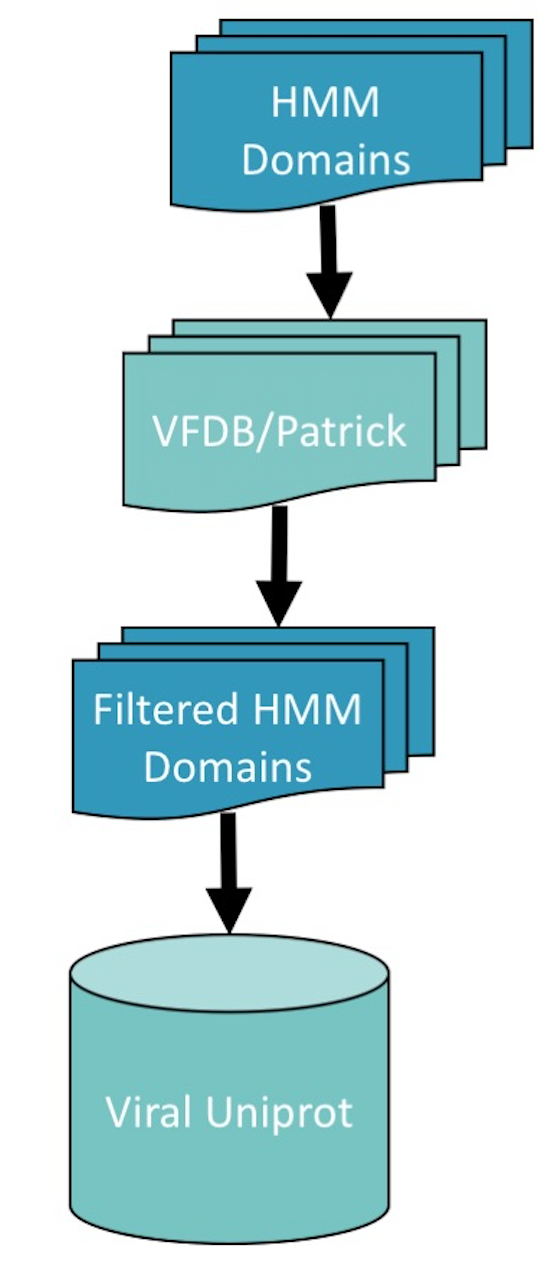
\includegraphics[height=6cm, width=3cm]{Pipeline.png}

	\end{columns}
	\end{frame}
	
	
	%-----------------------------------------	
	\begin{frame}{HMM Hit Distribution}
	\begin{columns}
	\column{0.6\textwidth}
	% Need to place figure
	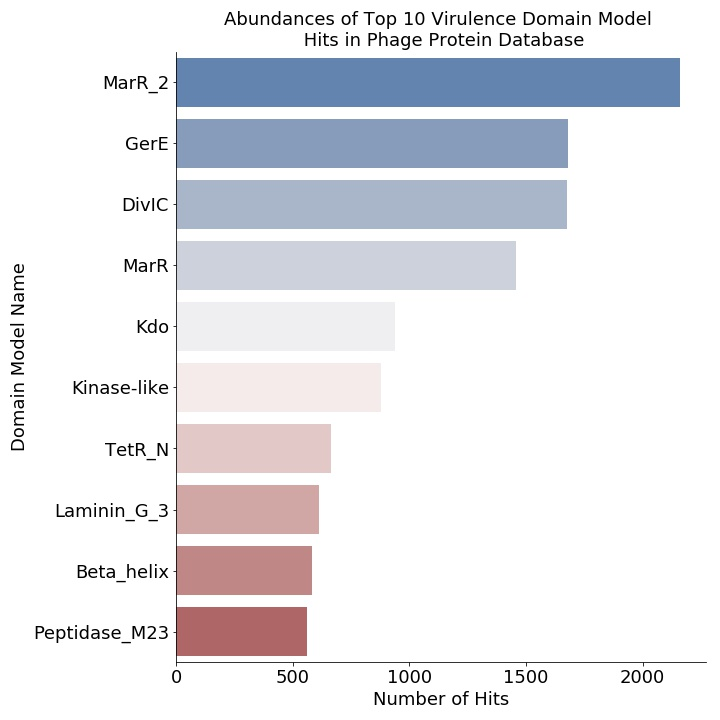
\includegraphics[height=6cm, width=6cm]{CPBS_11_18/TopDomains.jpg}
	\column{0.5\textwidth}
	\begin{block}{MarR\_2/MarR}
	Domain involved in antibiotic resistance
	\end{block}
	\begin{block}{DivIC}
	Part of sporulation process
	\end{block}
	\begin{block}{GerE}
	DNA binding domain found in virulence factors
	\end{block}
	\end{columns}
	\end{frame}
	
	%-----------------------------------------	
	\begin{frame}{Distribution of Hit Percentage in All Phages}
	\centering
	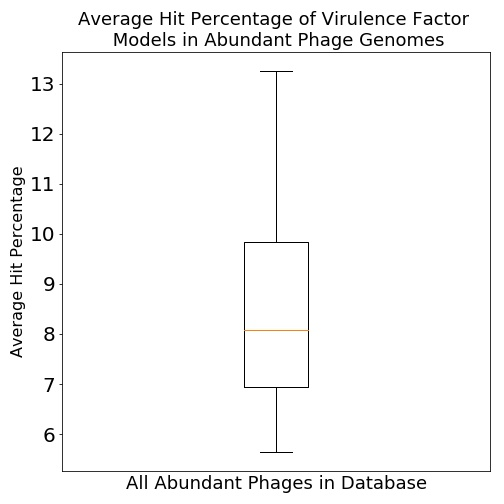
\includegraphics[height=7cm, width=7cm]{CPBS_11_18/AbundantPhageTotal.jpg}
	
	\end{frame}
	
	%-----------------------------------------	
	\begin{frame}{Abundant Phage Distributions by Genera Name}
	\centering
	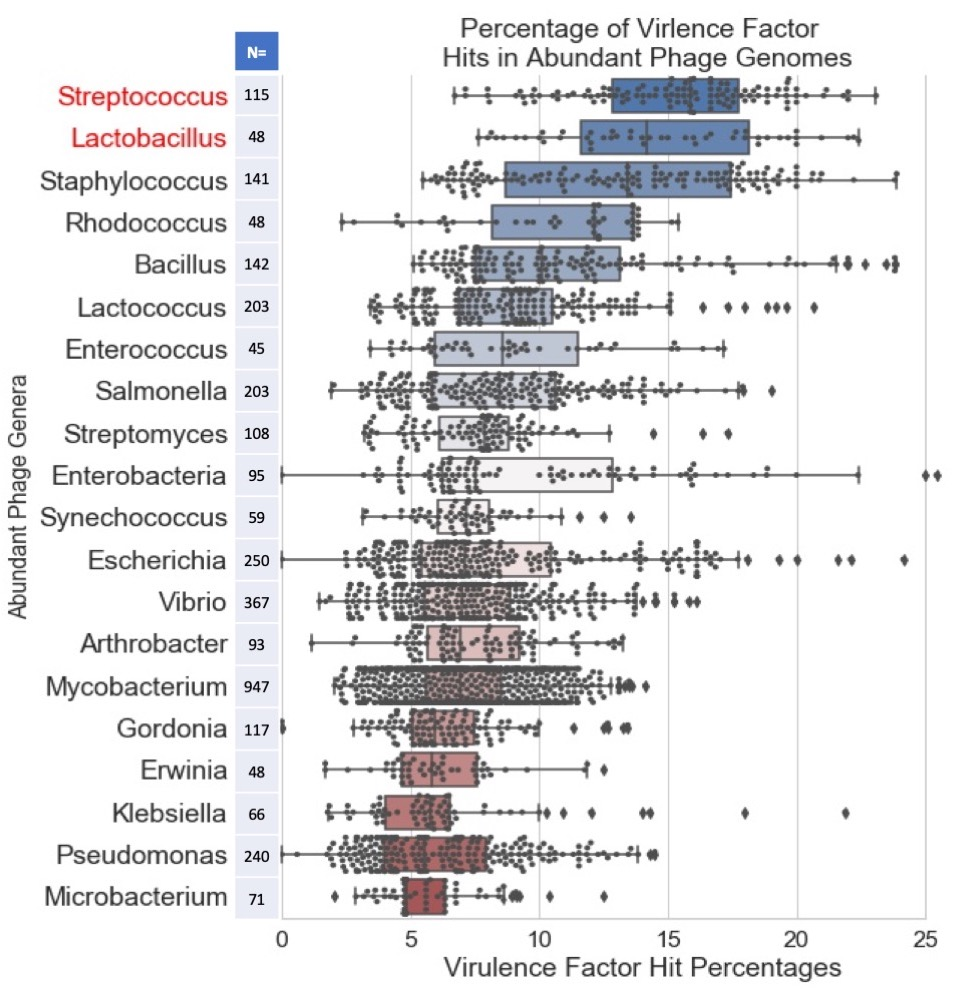
\includegraphics[height=7cm, width=8cm]{CPBS_11_18/Abundances.jpg}
	
	\end{frame}
	%-----------------------------------------	
	\begin{frame}{Random Set of PFAMs}
	\center
	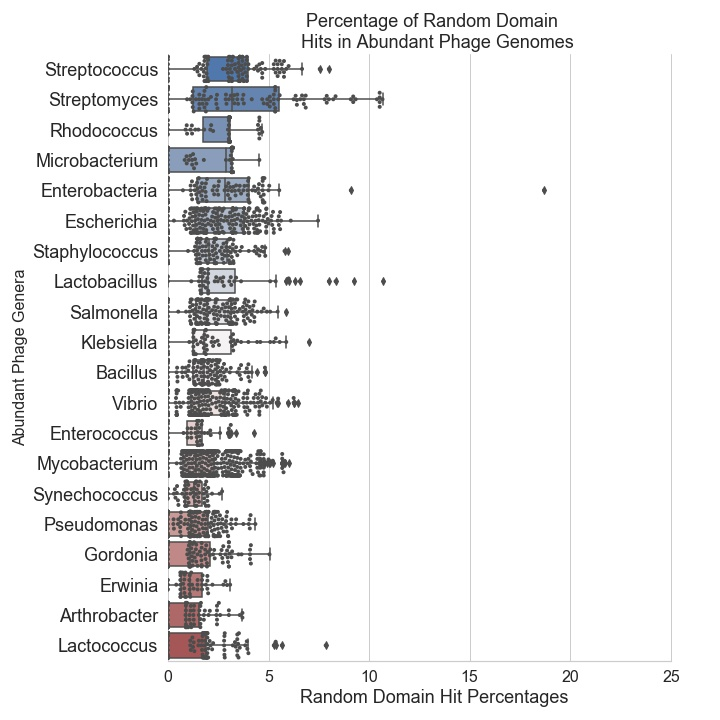
\includegraphics[height=7cm, width=10cm]{CPBS_11_18/Random.jpg}
	\end{frame}
	%-----------------------------------------	
	\begin{frame}{Full Top Domain Network}
	\center
	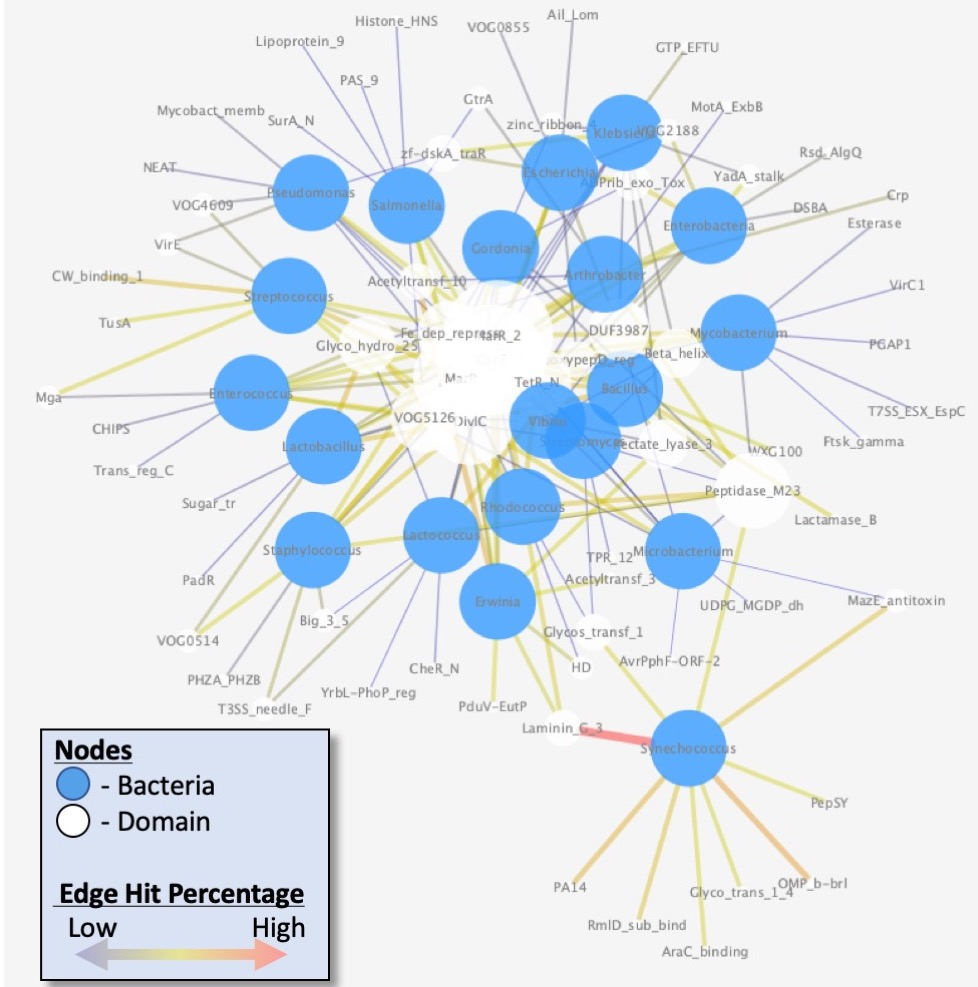
\includegraphics[height=7cm, width=10cm]{CPBS_11_18/Network.jpg}
	\end{frame}
	
	%-----------------------------------------
	\begin{frame}{Pathogen Subset Domain Network}
	\center
	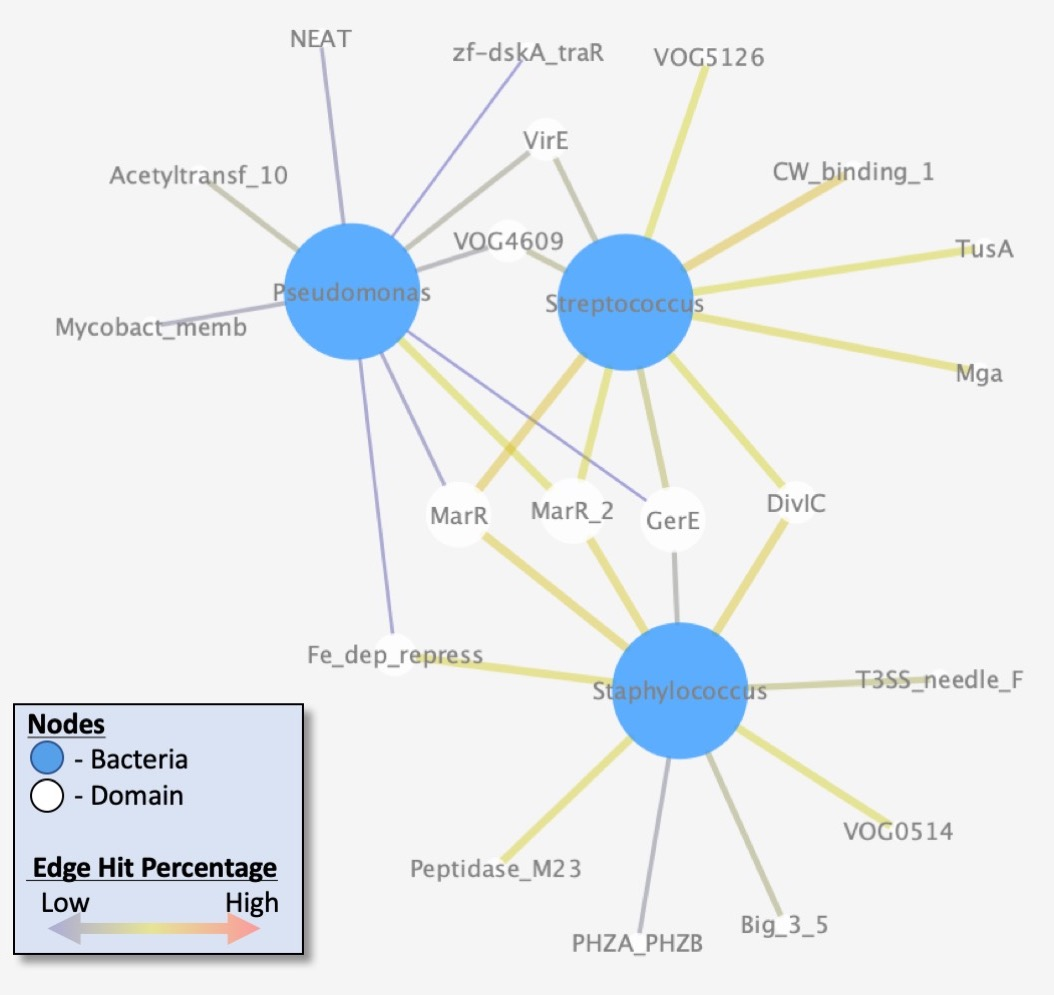
\includegraphics[height=7cm, width=10cm]{CPBS_11_18/Pathogenic.jpg}
	\end{frame}
	%-----------------------------------------
	\begin{frame}{Comparison to Integrated Phages from Clinical NTM}
  \center
	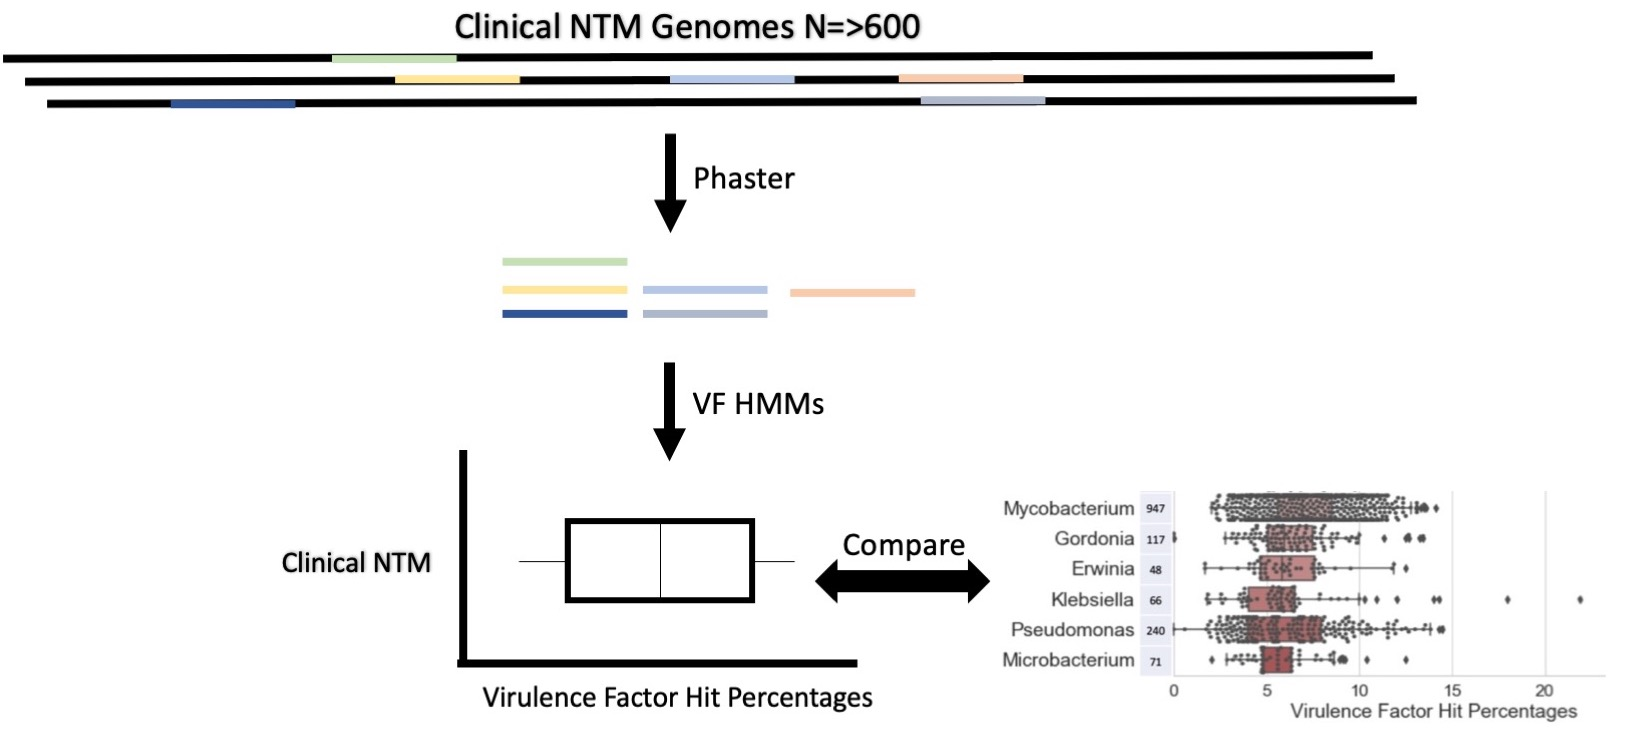
\includegraphics[height=7cm, width=10cm]{CPBS_11_18/ClinicalNTM.jpg} \\
	\tiny{Arndt, D., et al. Nucleic acids research (2016)}
	
	\end{frame}
	%------------------------------------------------------------------
	\begin{frame}{Conclusions and Future Directions}
	\begin{block}{Virulence Factors in Phages}
	Bacterial genera have different distributions of virulence factors in phage vectors
	\end{block}
	
	\begin{block}{Clinical Hypothesis Generation}
	The distribution of virulence factors in integrated phages can provide mechanisitic insight into clinical susceptibility and progression 
	\end{block}
	
	\end{frame}
	%------------------------------------------------------------------
	
	
\section{}
	\begin{frame}{Research Update Outline}
	\begin{block}{\textcolor{black!50}{Virulence Factors in Bacteriophages}}
	\textcolor{black!50}{\tiny{Glickman C., Hendrix J., Strong M. Computational identification and analysis of bacterial virulence factors embedded into bacteriophage genomes. Poster session accepted at: Rocky 18: 2018 Dec 8-10; Snowmass, CO}}
	\end{block}
	
	\begin{block}{Building Up Domains: Lysogenic Host Discovery}
  Incorporated into NCBI's Virus Discovery Project
	\end{block}

	\begin{block}{\textcolor{black!50}{Hybrid Viral Metagenome Prediction}}
	\textcolor{black!50}{\tiny{Glickman C., Strong M. Hybrid Viral Identification in Metagenomics. In preperation: Early 2019}}
	\end{block}
	\end{frame}
	
\section{Building Up Domains}
\subsection{}
	
	\begin{frame}{Endogenous Viral Elements (Prophages)}
	\begin{block}{Lysogenic Life Cycle}
	Viruses can integrate into host for an extended period of time
	\center
	\vspace{-0.2cm}
	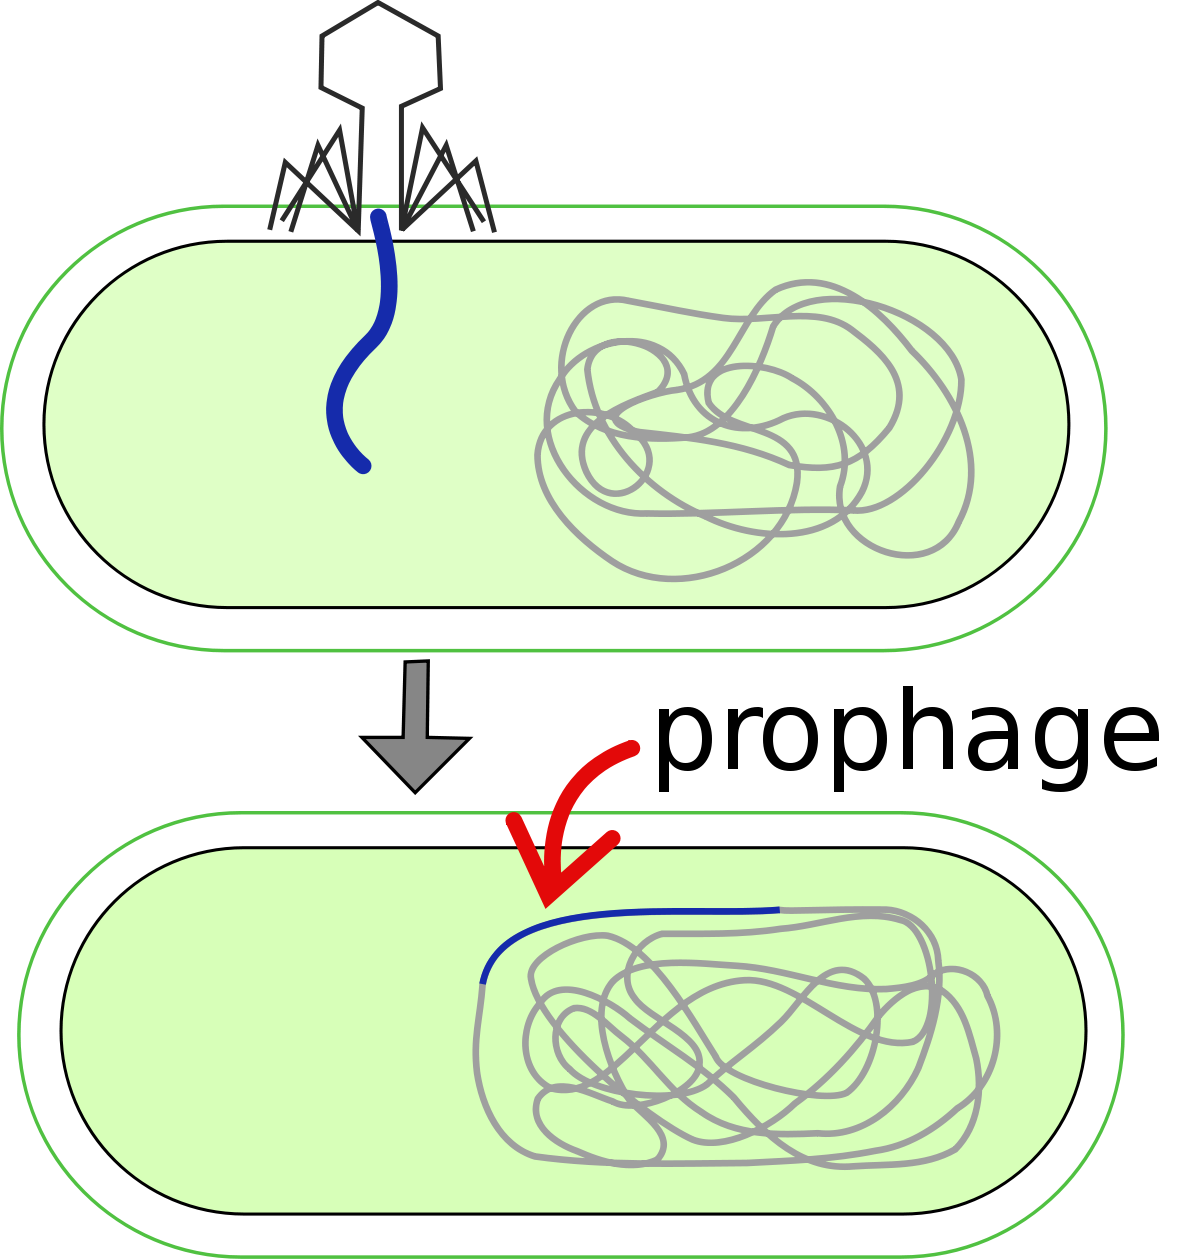
\includegraphics[height=3.5cm, width=5cm]{prophage.png}
	\end{block}
	\begin{block}{Importance of Prophages}
	Prophages can confer advantages to host improving survival \\ 
	Prophages are important to the emergence of pathogenic bacteria
	\end{block}
	
	\tiny{Canchaya C., et al. Curr Opin Microbiol (2003) \\ Wagner PL. \& Waldor MK. Infect Immune (2002)}
	\end{frame}
%------------------------------------------------------------------
	\begin{frame}{Finding Prophages}
	\begin{block}{Prophage Discovery Problem}
	Same difficulties as gene prediction: finding signal in data
	\center
	
\includegraphics[height=4cm, width=5cm]{dna.png}
	\end{block}
	\end{frame}
%------------------------------------------------------------------	
	\begin{frame}{Prophage Discovery Tools}
	\begin{block}{Current Methods Use}
	\begin{itemize}
	\begin{columns}
	\column{0.5\textwidth}
	\item Sequence similarity
	\item Hidden Markov models 
	\item Transcription direction
	\column{0.5\textwidth}
	\item Protein length
	\item Sliding window GC content
	\item Phage specific kmer
	\end{columns}
	\end{itemize}
	\center
	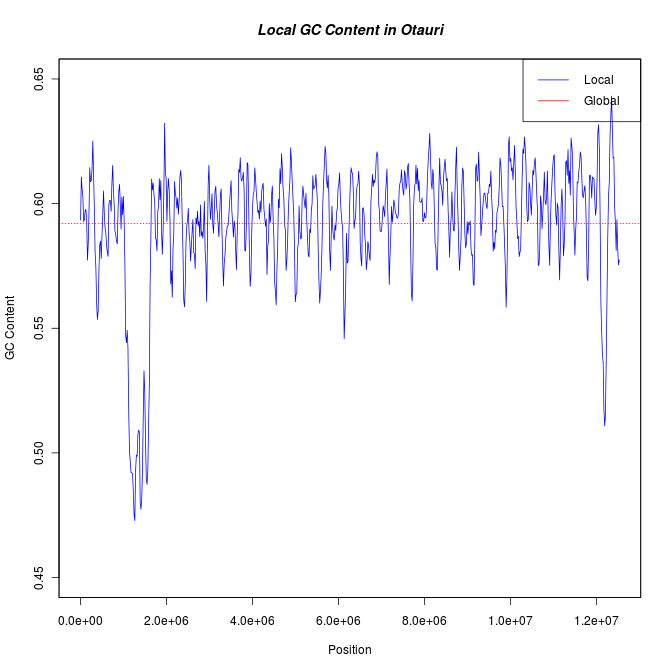
\includegraphics[height=5cm, width=7cm]{gc.png}
	\end{block}
	\end{frame}
	%------------------------------------------------------------------
	\begin{frame}{Prophage Discovery Methods}
	\begin{block}{Top Down Methods}
	All prophage discovery methods find prophages within contiguous sequences (contigs) or genomes
	\center
	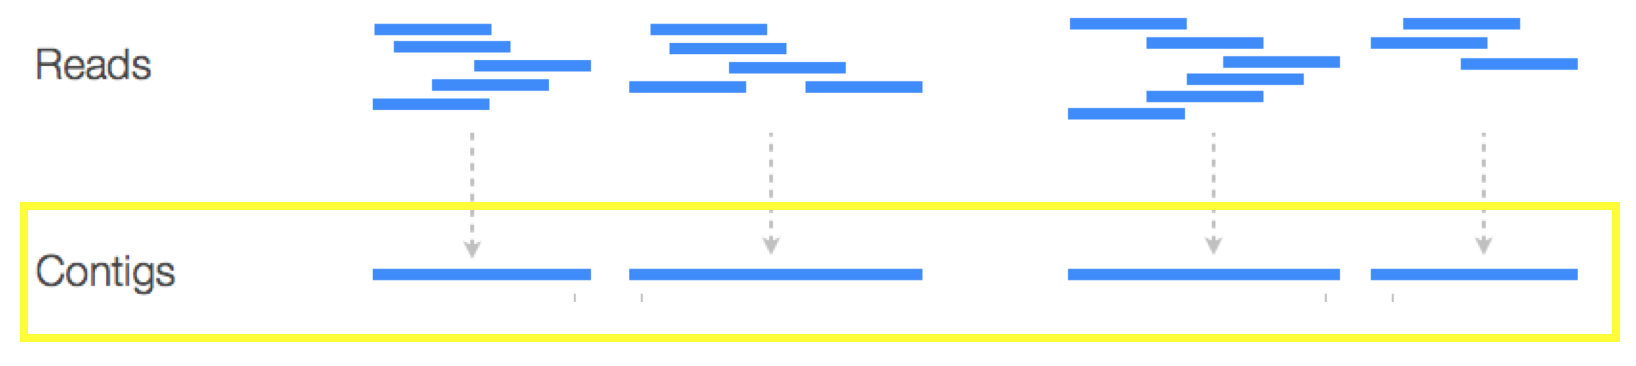
\includegraphics[height=3cm, width=5cm]{box_contigs.png}
	\end{block}
	
	
	\begin{block}{Top Down Pitfalls}
	Commonly require sequences longer than 1000 bases to make prediction with confidence
	\end{block}
	
	\end{frame}
	%------------------------------------------------------------------

	
	\begin{frame}{Building Up Domains (BUD) Algorithm}
	\begin{block}{Initialization}
	\begin{itemize}
	\item Metagenomic reads are filtered by BLAST against Viral RefSeq
	\item BLAST hits are assembled into contigs
	\end{itemize}
	\end{block}
	\vspace{-0.5cm}
	\center
	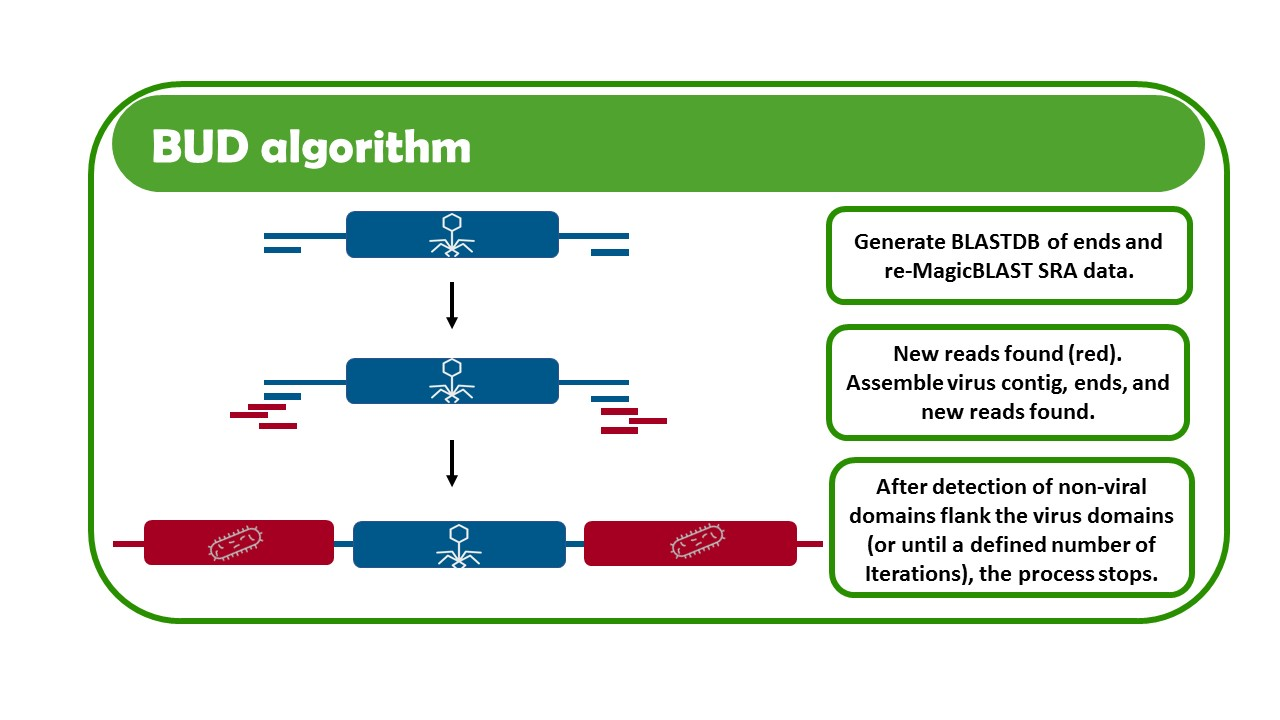
\includegraphics[height=6.75cm, width=10cm]{BUD_Algorithm.jpg}
	
	\end{frame}
	%------------------------------------------------------------------
	\begin{frame}{Potential Uses of BUD}

	\begin{block}{Expanding Known Phage Host Range}
	BUD has the potential to identify novel hosts for prophages
	
	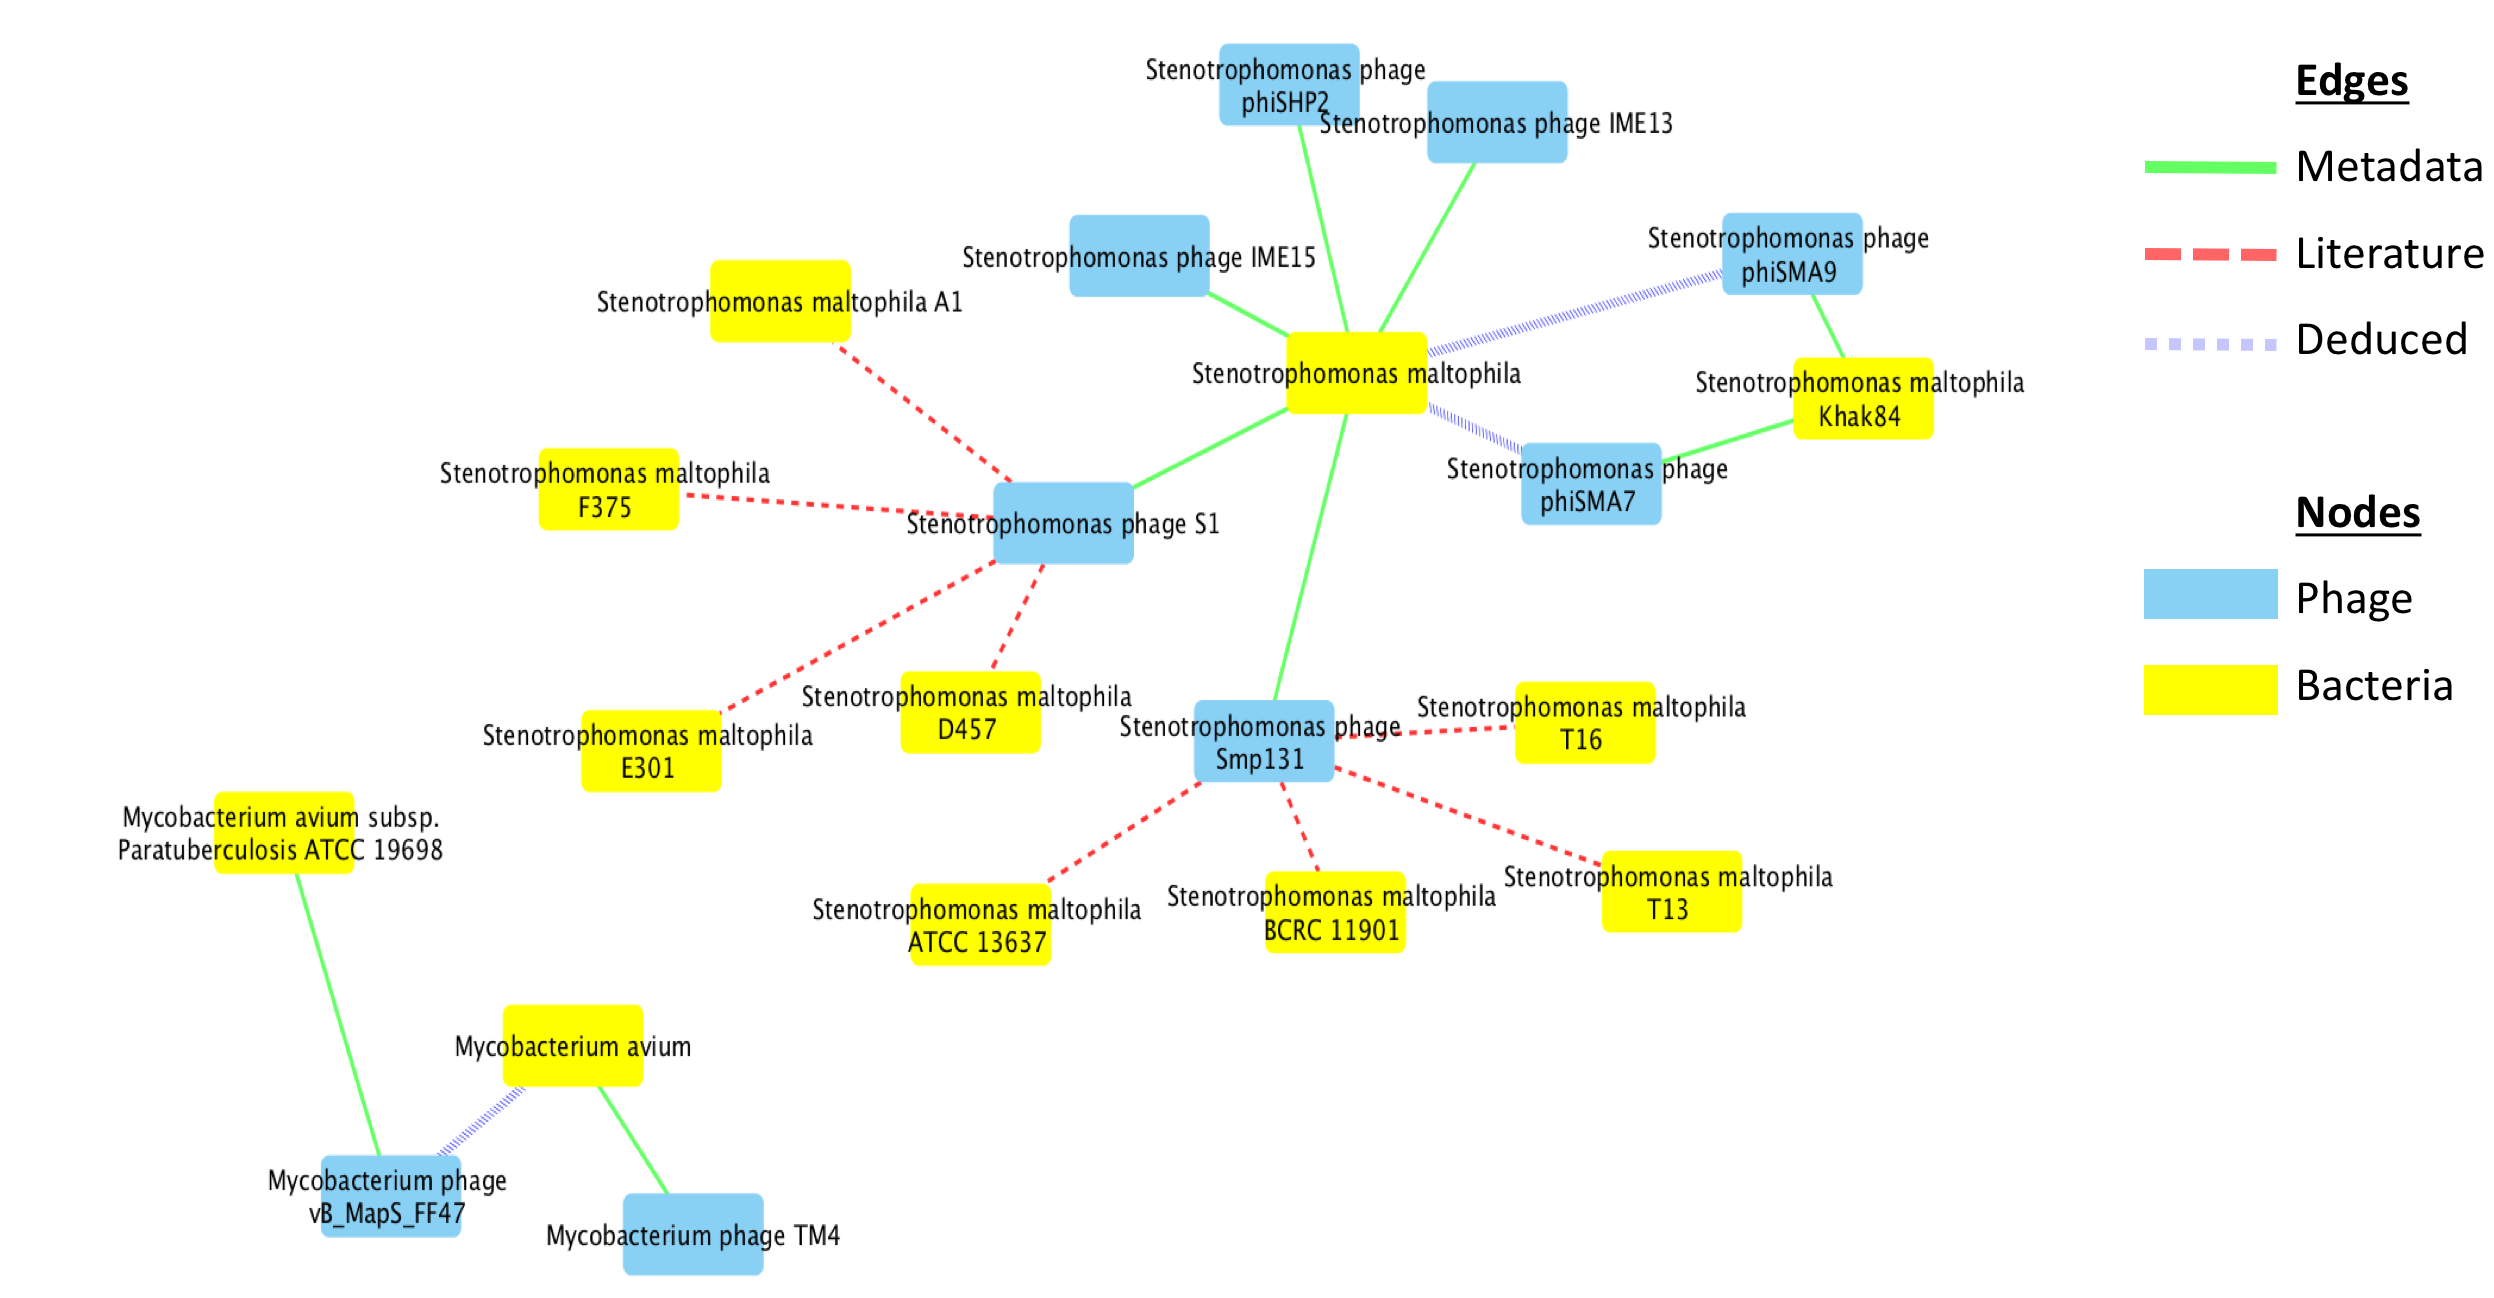
\includegraphics[height=6cm, width=11cm]{network.png}
	\end{block}
	
	\end{frame}
	%------------------------------------------------------------------
	\begin{frame}{Current Implementations of BUD}
	\begin{block}{ViruSpy}
	\begin{itemize}
	\item Originally written for NCBI Hackathon
	\item BUD Algorithm written in Perl and BASH

	\end{itemize}
	\end{block}
	
	\begin{block}{EndoVir}
	NCBI Collaborators Jan Buchman and Ben Busby \\ 
	\begin{itemize}
	\item Written in Python
	\item Implementation of BUD with Magic-BLAST
	\end{itemize}
	\end{block}
	\end{frame}
	%------------------------------------------------------------------
	\begin{frame}{Future Directions}
	\begin{block}{Overlap Consensus BUD}
	Create a version of BUD for local metagenomic sequences 
	\end{block}
	
	\begin{block}{Viral Discovery Project (VDP)}
	Integration into VDP a large collaboration aimed at renovating Viral Refseq and provide viral research protocol standards
	\end{block}
	\end{frame}
	%------------------------------------------------------------------
	
\section{}
%------------------------------------------------------------------ Outline
	\begin{frame}{Research Update Outline}
	\begin{block}{\textcolor{black!50}{Virulence Factors in Bacteriophages}}
	\textcolor{black!50}{\tiny{Glickman C., Hendrix J., Strong M. Computational identification and analysis of bacterial virulence factors embedded into bacteriophage genomes. Poster session accepted at: Rocky 18: 2018 Dec 8-10; Snowmass, CO}}
	\end{block}
	
	\begin{block}{\textcolor{black!50}{Building Up Domains: Lysogenic Host Discovery}}
  \textcolor{black!50}{Incorporated into NCBI's Virus Discovery Project}
	\end{block}

	\begin{block}{Hybrid Viral Contig Prediction}
	\tiny{Glickman C., Strong M. Hybrid Viral Identification in Metagenomics. In preperation: Early 2019}
	\end{block}
	\end{frame}
	
%------------------------------------------------------------------
	
\section{Hybrid Viral Contig Prediction}
\subsection{}

%-------------------------------------
  \begin{frame}{Metagenomics}
	\begin{columns}
	\column{0.5\textwidth}
	\begin{block}{What is Metagenomics?}
	Unbiased study of all genetic material in a sample
	\end{block}
	\begin{block}{Importance of Metagenomics}
	\begin{itemize}
	\item Functional capabilities of a sample
	\item Species level distinctions
	\item Due to lack of a universal gene marker, phages are studied by metagenomics
	\end{itemize}
	\end{block}
	
	\column{0.5\textwidth}
	
\includegraphics[height=5.5cm, width=5cm]{mosaic.png}
	\end{columns}
	\end{frame}

%-------------------------------------
  \begin{frame}{Methods to Isolate Phages in Metagenomics}
  \begin{block}{Biological Isolations}
  Filtrations and density gradiants to collect small particles \\
  {\tiny Lim, Y.W., et al. JoVE (2014)}
  \end{block}
  \begin{block}{Sequence Similarity}
  Mapping to genomes, BLAST, and Hidden Markov Models \\ 
  {\tiny Roux, S., et al. PeerJ (2015)}
  \end{block}
  \begin{block}{Machine Learning Methods}
  Linear discriminant analysis classifier on sequence k-mer profiles \\
  {\tiny Ren, Jie, et al. Microbiome (2017)}
  \end{block}
  \end{frame}
  %------------------------------------------------------------------
  \begin{frame}{Current Tool Limitations}
  \begin{block}{Sequence Similarity}
  \begin{itemize}
  \item Accessibility of top performing tool is limited to integrated environment
  \item Requires sequences to be longer than 1000 nucleotides \\
  {\tiny Roux, S., et al. PeerJ (2015)}
  \end{itemize}
  \end{block}
  \begin{block}{Machine Learning Methods}
  \begin{itemize}
  \item Isolated to R framework
  \item Performance is similar to sequence similarity with longer contigs \\
  {\tiny Ren, Jie, et al. Microbiome (2017)}
  \end{itemize}
  \end{block}
  \end{frame}
  %------------------------------------------------------------------
  %------------------------------------------------------------------
  \begin{frame}{Two-Step Hybrid Model}
  \center
	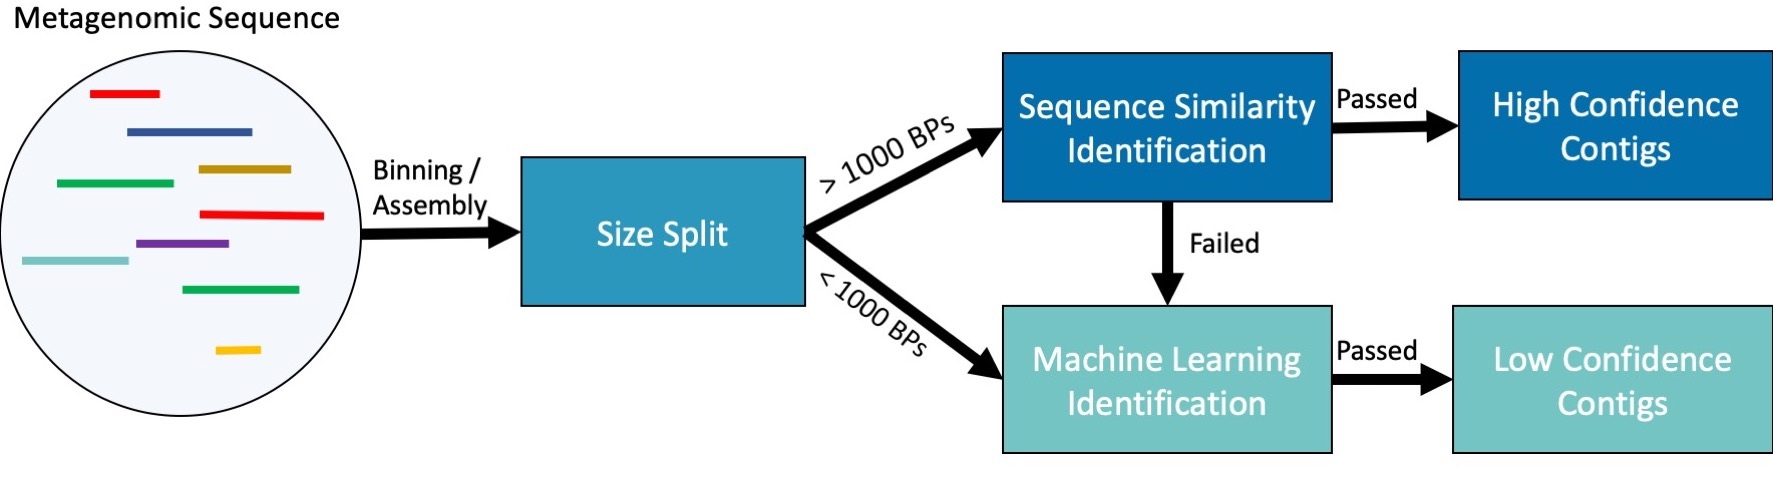
\includegraphics[height=4cm, width=10cm]{CPBS_11_18/TwoStep.jpg}
  
  \end{frame}
  %------------------------------------------------------------------
  \begin{frame}{Methods}
  HMMs from Earth Virome
  
  Python developed model with standalone operability
  
  \end{frame}
%------------------------------------------------------------------
  \begin{frame}{Comparison}
  Performance Comparison Using Critical Assessment of Metagenome Interpretation (CAMI) Data
  
  
  
  \tiny{Sczyrba, A., et al. Nature Methods (2017)}
	\end{frame}
	
	%------------------------------------------------------------------
	\begin{frame}{Future Directions}

	\end{frame}
%------------------------------------------------------------------
\section{}
	
	\begin{frame}{Concluding Remarks}
	\begin{columns}
	\column{0.3\textwidth}
	\begin{block}{Virulence Factors in Bacteriophages}
	Characterized bacterial virulence factors within phage vectors and compared distribution in database to clinical cohort
	\end{block}
	\column{0.3\textwidth}
	\begin{block}{Building Up Domains: Lysogenic Host Discovery}
	A bottom up approach to identifiying lysogenic phages within metagenomics
	\end{block}
	\column{0.3\textwidth}
	\begin{block}{Hybrid Viral Contig Prediction}
	An accessible two-step hybrid viral prediction pipeline for viral identification in metagenomics
	\end{block}
	
	\end{columns}
	
	\end{frame}
	
	%------------------------------------------------------------------
	
	
	\begin{frame}{Acknowledgements}
	\center
	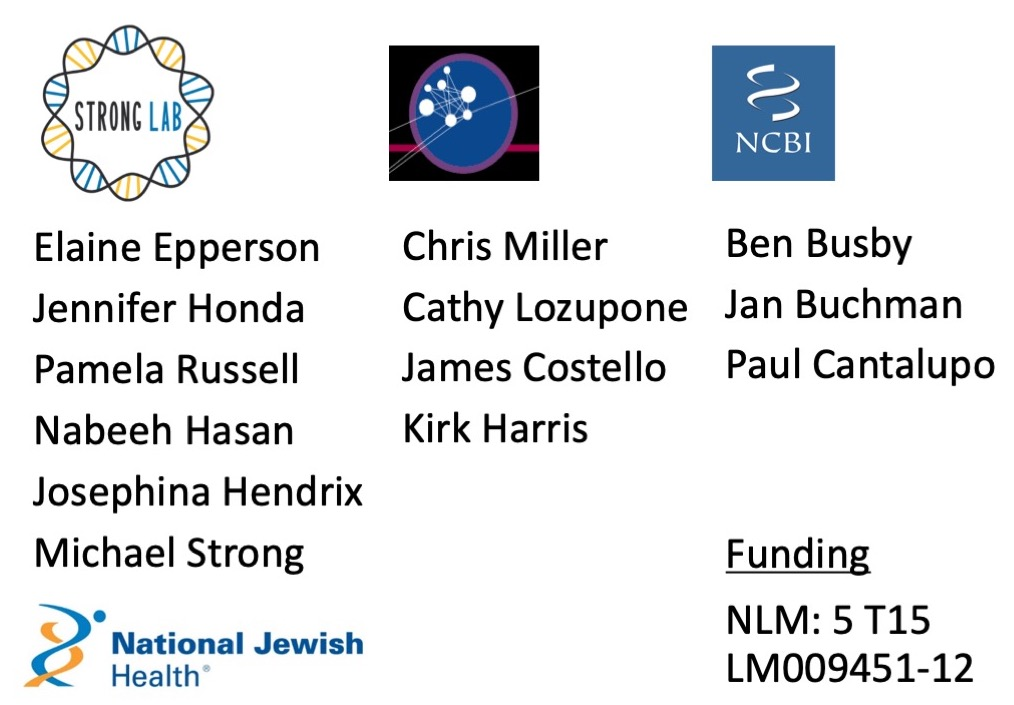
\includegraphics[height=7cm, width=10cm]{CPBS_11_18/Acknowledgements.jpg}
	\end{frame}
	%------------------------------------------------------------------
	
	\begin{frame}{Questions?}
	\center
	Cody Glickman \\ 
\includegraphics[height=2cm, width=2cm]{lablogo.png} \\ cody.glickman@ucdenver.edu \\ \alert{www.github.com/glickmac} \\ www.codyglickman.com
	\end{frame}
	%------------------------------------------------------------------

	
	
\end{document}